\documentclass{article}

\usepackage{minted}
\usepackage[most]{tcolorbox}
\usepackage{geometry}
\usepackage{enumitem}
\usepackage{hyperref}
\usepackage{hyperref}
\usepackage[parfill]{parskip}
\usepackage{wrapfig}
\usepackage{accsupp}

\geometry{margin=0.8in}
\definecolor{lightgreen}{rgb}{0.56, 0.93, 0.56}
\definecolor{moonstoneblue}{rgb}{0.45, 0.66, 0.76}
\definecolor{magenta}{rgb}{0.8,0.66,0.76}
\begin{document}
\BeginAccSupp{}
\begin{flushright}
Computational Biology ~\\
Tufts University Bio 35 ~\\
Fall 2021 ~\\ ~\\
\end{flushright}
\begin{center}{\textbf{\Large{Spotlight 10: Ambika Kamath}}}\end{center}

\textit{Please note that in general I have taken/adapted the words of our Spotlight subjects from their own websites to describe their work. I have done this in an effort to maintain accuracy in describing their research programs. Please do not copy paste text from their papers/websites in your assignments!}

\begin{wrapfigure}{L}{0.14\textwidth}
\begin{center}
 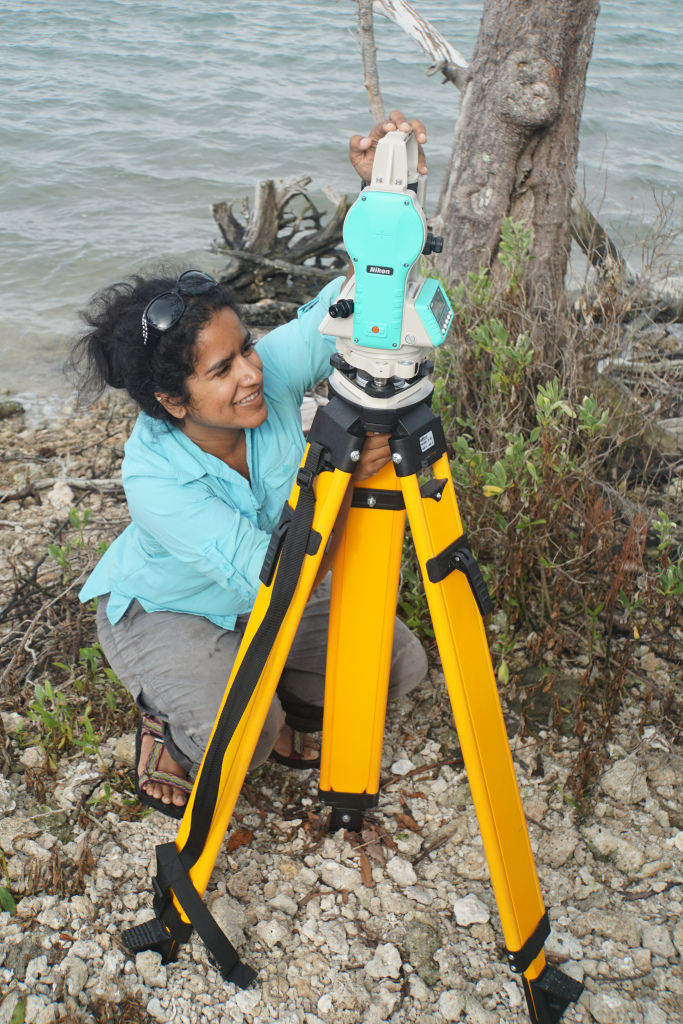
\includegraphics[width=0.13\textwidth]{images/ambika-kamath.jpeg}
 \end{center}
\end{wrapfigure}
~\\ As part of our unit on evolutionary inferences, we are going to explore the work of Ambika Kamath. Prof. Kamath's lab studies how and why animals interact with one another and with their environments, and the ecological and evolutionary consequences of these interactions. Their overarching goal is to understand how behavior both shapes and is shaped by ecological and evolutionary forces. They also take seriously the idea that human identities, perspectives and biases influence and are influenced by animal behavior. Dr. Kamath is a Professor at the University of Colorado.
~\\ ~\\

Please read the following article, on which Prof. Kamath is a co-author: 
\begin{enumerate}
\item \texttt{\href{https://www.nature.com/articles/s41559-019-1019-7.pdf}{https://www.nature.com/articles/s41559-019-1019-7.pdf}}
\end{enumerate}

Also listen to the following podcast:
\begin{enumerate}
\item \texttt{\href{https://soundcloud.com/sse-communications/ambika-kamath-story-collider-evolution-2019}{https://soundcloud.com/sse-communications/ambika-kamath-story-collider-evolution-2019}}
\end{enumerate}

\subsubsection*{Written Assignment} 
After reading Ambika Kamath's article and listening to the podcast, write a reflection (max one page) on what you discovered. You might wish to address some of the following: 

\begin{enumerate}
\item What was most interesting to you in reviewing these resources?
\item What did you learn from these resources about the scientific process or the ability of genetic data to inform or overturn scientific theories? How might the implementation or interpretation of computational tools be affected by identity or social context?
\item What new questions do you have after reviewing these resources?
\item What do these resources tell you about the types of people that do computational biology, or their motivations?
\end{enumerate}

\EndAccSupp{}
\end{document}